% Native PGFPlots; generated by examples/generate_figures.py.
% Constructed or analytical teaching example.
\begingroup
\definecolor{blueplot}{HTML}{4E79A7}
\definecolor{redplot}{HTML}{D95F59}
\definecolor{inkplot}{HTML}{111111}
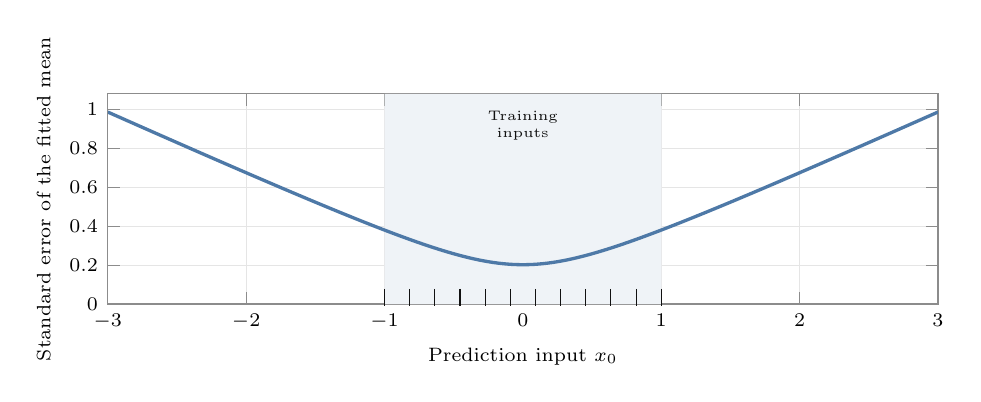
\begin{tikzpicture}
\begin{axis}[
width=\linewidth,height=4.25cm,font=\scriptsize,
tick label style={font=\scriptsize},label style={font=\scriptsize},
axis line style={black!45},tick style={black!45},
grid=major,grid style={black!10},scaled ticks=false,
clip=true,unbounded coords=jump,
legend style={font=\tiny,draw=none,fill=white,fill opacity=.94,text opacity=1,
  legend cell align=left,inner sep=2pt,row sep=1pt},
xmin=-3,xmax=3,ymin=0,ymax=1.08,
xlabel={Prediction input $x_0$},ylabel={Standard error of the fitted mean},
xtick={-3,-2,-1,0,1,2,3},ytick={0,.2,.4,.6,.8,1},
]
\addplot[draw=none,fill=blueplot!9,forget plot] coordinates {(-1,0) (1,0) (1,1.08) (-1,1.08)} \closedcycle;
\addplot[blueplot,very thick,no marks] coordinates {(-3,0.9867714775) (-2.98,0.9804697592) (-2.96,0.9741698372) (-2.94,0.9678717466) (-2.92,0.9615755234) (-2.9,0.9552812044) (-2.88,0.9489888276) (-2.86,0.9426984318) (-2.84,0.936410057) (-2.82,0.9301237442) (-2.8,0.9238395354) (-2.78,0.9175574739) (-2.76,0.9112776041) (-2.74,0.9049999717) (-2.72,0.8987246234) (-2.7,0.8924516075) (-2.68,0.8861809736) (-2.66,0.8799127725) (-2.64,0.8736470566) (-2.62,0.8673838798) (-2.6,0.8611232974) (-2.58,0.8548653665) (-2.56,0.8486101458) (-2.54,0.8423576955) (-2.52,0.8361080779) (-2.5,0.829861357) (-2.48,0.8236175986) (-2.46,0.8173768707) (-2.44,0.8111392432) (-2.42,0.8049047881) (-2.4,0.7986735799) (-2.38,0.792445695) (-2.36,0.7862212124) (-2.34,0.7800002137) (-2.32,0.7737827827) (-2.3,0.7675690063) (-2.28,0.7613589739) (-2.26,0.7551527779) (-2.24,0.7489505136) (-2.22,0.7427522795) (-2.2,0.7365581774) (-2.18,0.7303683124) (-2.16,0.7241827932) (-2.14,0.718001732) (-2.12,0.711825245) (-2.1,0.7056534524) (-2.08,0.6994864783) (-2.06,0.6933244514) (-2.04,0.6871675047) (-2.02,0.681015776) (-2,0.6748694081) (-1.98,0.6687285487) (-1.96,0.6625933509) (-1.94,0.6564639737) (-1.92,0.6503405814) (-1.9,0.6442233448) (-1.88,0.6381124409) (-1.86,0.6320080533) (-1.84,0.6259103729) (-1.82,0.6198195974) (-1.8,0.6137359325) (-1.78,0.6076595918) (-1.76,0.6015907971) (-1.74,0.5955297792) (-1.72,0.589476778) (-1.7,0.5834320429) (-1.68,0.5773958337) (-1.66,0.5713684204) (-1.64,0.5653500844) (-1.62,0.5593411188) (-1.6,0.5533418288) (-1.58,0.5473525325) (-1.56,0.5413735617) (-1.54,0.5354052623) (-1.52,0.5294479951) (-1.5,0.5235021367) (-1.48,0.5175680805) (-1.46,0.511646237) (-1.44,0.5057370351) (-1.42,0.4998409234) (-1.4,0.4939583705) (-1.38,0.4880898667) (-1.36,0.4822359248) (-1.34,0.4763970817) (-1.32,0.4705738995) (-1.3,0.4647669667) (-1.28,0.4589769002) (-1.26,0.4532043463) (-1.24,0.4474499829) (-1.22,0.4417145209) (-1.2,0.4359987062) (-1.18,0.4303033218) (-1.16,0.4246291897) (-1.14,0.4189771734) (-1.12,0.41334818) (-1.1,0.4077431633) (-1.08,0.4021631255) (-1.06,0.396609121) (-1.04,0.391082259) (-1.02,0.3855837067) (-1,0.3801146925) (-0.98,0.37467651) (-0.96,0.3692705214) (-0.94,0.3638981613) (-0.92,0.3585609414) (-0.9,0.3532604545) (-0.88,0.347998379) (-0.86,0.3427764839) (-0.84,0.3375966338) (-0.82,0.3324607939) (-0.8,0.3273710355) (-0.78,0.3223295415) (-0.76,0.3173386123) (-0.74,0.3124006714) (-0.72,0.3075182713) (-0.7,0.3026940996) (-0.68,0.297930985) (-0.66,0.2932319026) (-0.64,0.2885999805) (-0.62,0.2840385041) (-0.6,0.2795509219) (-0.58,0.2751408497) (-0.56,0.2708120741) (-0.54,0.2665685557) (-0.52,0.2624144305) (-0.5,0.2583540108) (-0.48,0.2543917835) (-0.46,0.2505324074) (-0.44,0.2467807082) (-0.42,0.2431416702) (-0.4,0.2396204263) (-0.38,0.2362222443) (-0.36,0.2329525097) (-0.34,0.2298167051) (-0.32,0.2268203853) (-0.3,0.2239691485) (-0.28,0.2212686034) (-0.26,0.2187243318) (-0.24,0.2163418473) (-0.22,0.2141265502) (-0.2,0.2120836797) (-0.18,0.2102182626) (-0.16,0.2085350613) (-0.14,0.2070385199) (-0.12,0.2057327118) (-0.1,0.2046212887) (-0.08,0.2037074322) (-0.06,0.2029938107) (-0.04,0.2024825412) (-0.02,0.2021751589) (0,0.2020725942) (0.02,0.2021751589) (0.04,0.2024825412) (0.06,0.2029938107) (0.08,0.2037074322) (0.1,0.2046212887) (0.12,0.2057327118) (0.14,0.2070385199) (0.16,0.2085350613) (0.18,0.2102182626) (0.2,0.2120836797) (0.22,0.2141265502) (0.24,0.2163418473) (0.26,0.2187243318) (0.28,0.2212686034) (0.3,0.2239691485) (0.32,0.2268203853) (0.34,0.2298167051) (0.36,0.2329525097) (0.38,0.2362222443) (0.4,0.2396204263) (0.42,0.2431416702) (0.44,0.2467807082) (0.46,0.2505324074) (0.48,0.2543917835) (0.5,0.2583540108) (0.52,0.2624144305) (0.54,0.2665685557) (0.56,0.2708120741) (0.58,0.2751408497) (0.6,0.2795509219) (0.62,0.2840385041) (0.64,0.2885999805) (0.66,0.2932319026) (0.68,0.297930985) (0.7,0.3026940996) (0.72,0.3075182713) (0.74,0.3124006714) (0.76,0.3173386123) (0.78,0.3223295415) (0.8,0.3273710355) (0.82,0.3324607939) (0.84,0.3375966338) (0.86,0.3427764839) (0.88,0.347998379) (0.9,0.3532604545) (0.92,0.3585609414) (0.94,0.3638981613) (0.96,0.3692705214) (0.98,0.37467651) (1,0.3801146925) (1.02,0.3855837067) (1.04,0.391082259) (1.06,0.396609121) (1.08,0.4021631255) (1.1,0.4077431633) (1.12,0.41334818) (1.14,0.4189771734) (1.16,0.4246291897) (1.18,0.4303033218) (1.2,0.4359987062) (1.22,0.4417145209) (1.24,0.4474499829) (1.26,0.4532043463) (1.28,0.4589769002) (1.3,0.4647669667) (1.32,0.4705738995) (1.34,0.4763970817) (1.36,0.4822359248) (1.38,0.4880898667) (1.4,0.4939583705) (1.42,0.4998409234) (1.44,0.5057370351) (1.46,0.511646237) (1.48,0.5175680805) (1.5,0.5235021367) (1.52,0.5294479951) (1.54,0.5354052623) (1.56,0.5413735617) (1.58,0.5473525325) (1.6,0.5533418288) (1.62,0.5593411188) (1.64,0.5653500844) (1.66,0.5713684204) (1.68,0.5773958337) (1.7,0.5834320429) (1.72,0.589476778) (1.74,0.5955297792) (1.76,0.6015907971) (1.78,0.6076595918) (1.8,0.6137359325) (1.82,0.6198195974) (1.84,0.6259103729) (1.86,0.6320080533) (1.88,0.6381124409) (1.9,0.6442233448) (1.92,0.6503405814) (1.94,0.6564639737) (1.96,0.6625933509) (1.98,0.6687285487) (2,0.6748694081) (2.02,0.681015776) (2.04,0.6871675047) (2.06,0.6933244514) (2.08,0.6994864783) (2.1,0.7056534524) (2.12,0.711825245) (2.14,0.718001732) (2.16,0.7241827932) (2.18,0.7303683124) (2.2,0.7365581774) (2.22,0.7427522795) (2.24,0.7489505136) (2.26,0.7551527779) (2.28,0.7613589739) (2.3,0.7675690063) (2.32,0.7737827827) (2.34,0.7800002137) (2.36,0.7862212124) (2.38,0.792445695) (2.4,0.7986735799) (2.42,0.8049047881) (2.44,0.8111392432) (2.46,0.8173768707) (2.48,0.8236175986) (2.5,0.829861357) (2.52,0.8361080779) (2.54,0.8423576955) (2.56,0.8486101458) (2.58,0.8548653665) (2.6,0.8611232974) (2.62,0.8673838798) (2.64,0.8736470566) (2.66,0.8799127725) (2.68,0.8861809736) (2.7,0.8924516075) (2.72,0.8987246234) (2.74,0.9049999717) (2.76,0.9112776041) (2.78,0.9175574739) (2.8,0.9238395354) (2.82,0.9301237442) (2.84,0.936410057) (2.86,0.9426984318) (2.88,0.9489888276) (2.9,0.9552812044) (2.92,0.9615755234) (2.94,0.9678717466) (2.96,0.9741698372) (2.98,0.9804697592) (3,0.9867714775)};
\addplot[only marks,mark=|,mark size=3pt,inkplot] coordinates {(-1,0.035) (-0.8181818182,0.035) (-0.6363636364,0.035) (-0.4545454545,0.035) (-0.2727272727,0.035) (-0.09090909091,0.035) (0.09090909091,0.035) (0.2727272727,0.035) (0.4545454545,0.035) (0.6363636364,0.035) (0.8181818182,0.035) (1,0.035)};
\node[font=\tiny,align=center,anchor=north,text=inkplot] at (axis cs:0,1.04) {Training\\inputs};

\end{axis}
\end{tikzpicture}
\endgroup
